\chapter{Bitshield}
\label{chap:arc}

\section{System model}

\section{Information dissemination}

\subsection{Neighbours ordering}
\label{sec:propagacao}

To solve the problem referenced in Section~\ref{} NAME takes advantage of asymmetries that already exists in the network. Namely the fact that the majority of blocks are mainly mined by mining pools with only a total of 11 (7.6\%) blocks mined in a day coming from unknown sources.

With this information, the objective of NAME is to prioritize miners in the process of dissemination. To be able to do this the nodes have to discover the best path to the closest miners. Here the best path is the path that takes less time for the transactions of a node to reach a miner. We achieve this by ordering our neighbours by proximity to miners. Hence, the neighbours closest to miners will be on top of our ordering and the ones further away will be at the bottom.

To obtain this classification of neighbours each node will maintain for each neighbour five variables:
\begin{itemize}
  \item \textit{n} total number of blocks received by that neighbour;
  \item \textit{k} accumulated time it took to disseminate a block to us;
  \item \textit{a} total number of blocks received;
  \item \textit{z} total number of transactions we sent to that neighbour;
  \item \textit{y} accumulated time it took for those transactions to be accepted in a block.
\end{itemize}

The time it takes for a neighbour to relay a block until a node is given by the difference between the current time and the last time the node received a new block from that neighbour. If a neighbour takes more than four hours to relay a block to a node the difference will be the current time minus four hours.  If Given the large number of transactions that flow through the network, instead of maintaining timers for all of them we only maintain a timer each one hundred transactions. This way we do not overburden nodes with metadata.

\[ \mbox{class}^{T}= (\dfrac{k^{T}}{n^{T}} + a^{T} - n^{T} + \dfrac{y^{T}}{z^{T}}) \]

With this classification, we prevent nodes that only generate a block once in a while from having a good classification eternally.

This is important because as we have said, there is still a percentage of blocks being mined by random nodes, and if we would, for instance, send all our transactions to those nodes they would take a lot of time to appear in a block. Which is not desired, given that the average time it takes for a transaction to be accepted in Bitcoin nowadays is ten minutes.

This way for a neighbour to have good classification it has to have a good ratio of time it takes to disseminate blocks/number of blocks we received from him, a good ratio of blocks received from him/blocks received and finally a good ratio of time it took for a transaction to be added to blocks if we sent it to him.

Give that the classification of neighbours is prone to change over time, the actual value used to order neighbours is given by the following sliding average of the classification presented previously:

\[ \mbox{class}^t = (1-\alpha) \cdot \mbox{class}^{t-1} + \alpha \cdot \mbox{class}^{T} \]

The $\alpha$ factor exists to avoid nodes that once generated a lot of blocks but currently do not from having a good classification forever. In our experiments, we used an $\alpha=0.3$ and a \textit{T} configured to be an interval of four hours.

Each time a node receives a block from a neighbour the classification of that neighbour will be updated using Algorithm~\ref{alg:class}

\begin{algorithm}[t]
\begin{algorithmic}[1]
\Function{update\_nodes\_classificatoin}{node\_to\_update}
\State $\textit{new\_class} \gets \textit{recalculate\_class}(node\_to\_update)$
\State $\textit{worst\_class} \gets -1$
\State $\textit{worst\_node} \gets None$
\For{$node$ \textbf{in} $m$}
  \If{$new\_class =< node.class()$ \textbf{and} $worst\_class < node.class()$}
	\State $\textit{worst\_class} \gets \textit{node.class()}$
    \State $\textit{worst\_node} \gets \textit{node}$
    \EndIf
\EndFor
\If{$worst\_class != -1$}
	\State $\textit{m.remove}(worst\_node)$
    \State $\textit{m.append}(node\_to\_update)$
	\EndIf
\EndFunction
\end{algorithmic}
\caption{Best \textit{m} neighbours computation}
\label{alg:class}
\end{algorithm}
\vspace{-0.5cm}

\subsection{Skewed relay}
\label{sec:sr}
Give that our objective is that our transactions reach a miner as fast as possible we can use the mechanism described previously to do it. Hence, if all the nodes were to follow the protocol correctly, and the paths created by out solution were resilient enough we could send our transactions to only one node, and they would eventually appear in a block.

However, even if we do not consider the problem of nodes disconnecting from the network, there is the problem of time it takes for a transaction to be committed. So to solve this problem, we will send our transactions not only to the \textit{m} best nodes but also to \textit{a} random nodes, as it is described in Algorithm~\ref{alg:diss}. This way we assure that our transactions are still broadcast through the rest of the network and will be committed in a timely manner.

\begin{algorithm}[t]
\begin{algorithmic}[1]
\Function{nodes\_to\_send}{transaction}
\If{$m$ \textbf{is not} $empty$ \textbf{or} $(pi == True$ \textbf{and} $transaction.source() == self)$}
	\State {$\textbf{return}$ $neighbourhood$}
    \EndIf
\State $\textit{total} \gets \textit{size\_m} + \textit{size\_a}$
\State $\textit{best\_nodes} \gets \textit{m}$
\If{$size(neighbourhood) < total$}
	\State $\textit{total} \gets \textit{size(neighbourhood)} - \textit{size\_m}$
\Else
	\State $\textit{total} \gets \textit{total} - \textit{size\_m}$
    \EndIf
\If{$total > 0$}
	\State $\textit{random\_nodes} \gets \textit{random\_choise(neighbourhood, size\_a)}$
    \EndIf
\State \Return best\_nodes + random\_nodes
\EndFunction
\end{algorithmic}
\caption{Nodes to send transactions advertisements computation}
\label{alg:diss}
\end{algorithm}

The value of \acrshort{ip} indicates that if a transaction is generated by a node, the node has the option of either sending it for only \textit{m} plus \textit{a} or to all his neighbours.

Hence we can then configure the following variables \textit{size\_m}, \textit{size\_a} and \textit{ip} to obtain different results in the information dissemination. In Chapter~\ref{chap:evaluation} we will dicuss diferent configurations tested.

\section{Membership improvement}

\section{Implementation}


\section{Architecture}
\label{sec:arc}
Given the problems presented beforehand in this section, our goal is to build a set of extensions to Bitcoin and blockchain technologies to overcome these threats. We have chosen Bitcoin to implement these extensions because it not only has a big user base but it also well documented and has been the focus of many research articles. Whereas other cryptocurrencies do not usually have proper documentation of the protocols they use and their code. With this lack of information, it would be difficult to identify the key modules that we would need to modify or improve to create these extensions for those cryptocurrencies.

As we have seen Bitcoin still has a lot of problems linked to the network protocol and the overlay used, that the other cryptocurrencies do not have. It is worth noticing that those cryptocurrencies like Ripple, for instance, sacrifice other properties in exchange for being protected against those vulnerabilities, for instance, connections in Ripple are encrypted which imposes an overhead on the nodes. Therefore, in this work we propose to extend Bitcoin architecture with a module, which we call BitShield, to address these problems while also having a low impact on performance. The architecture is presented in Fig. \ref{fig:bitshieldoverview}.

\begin{figure}[h]
\centering
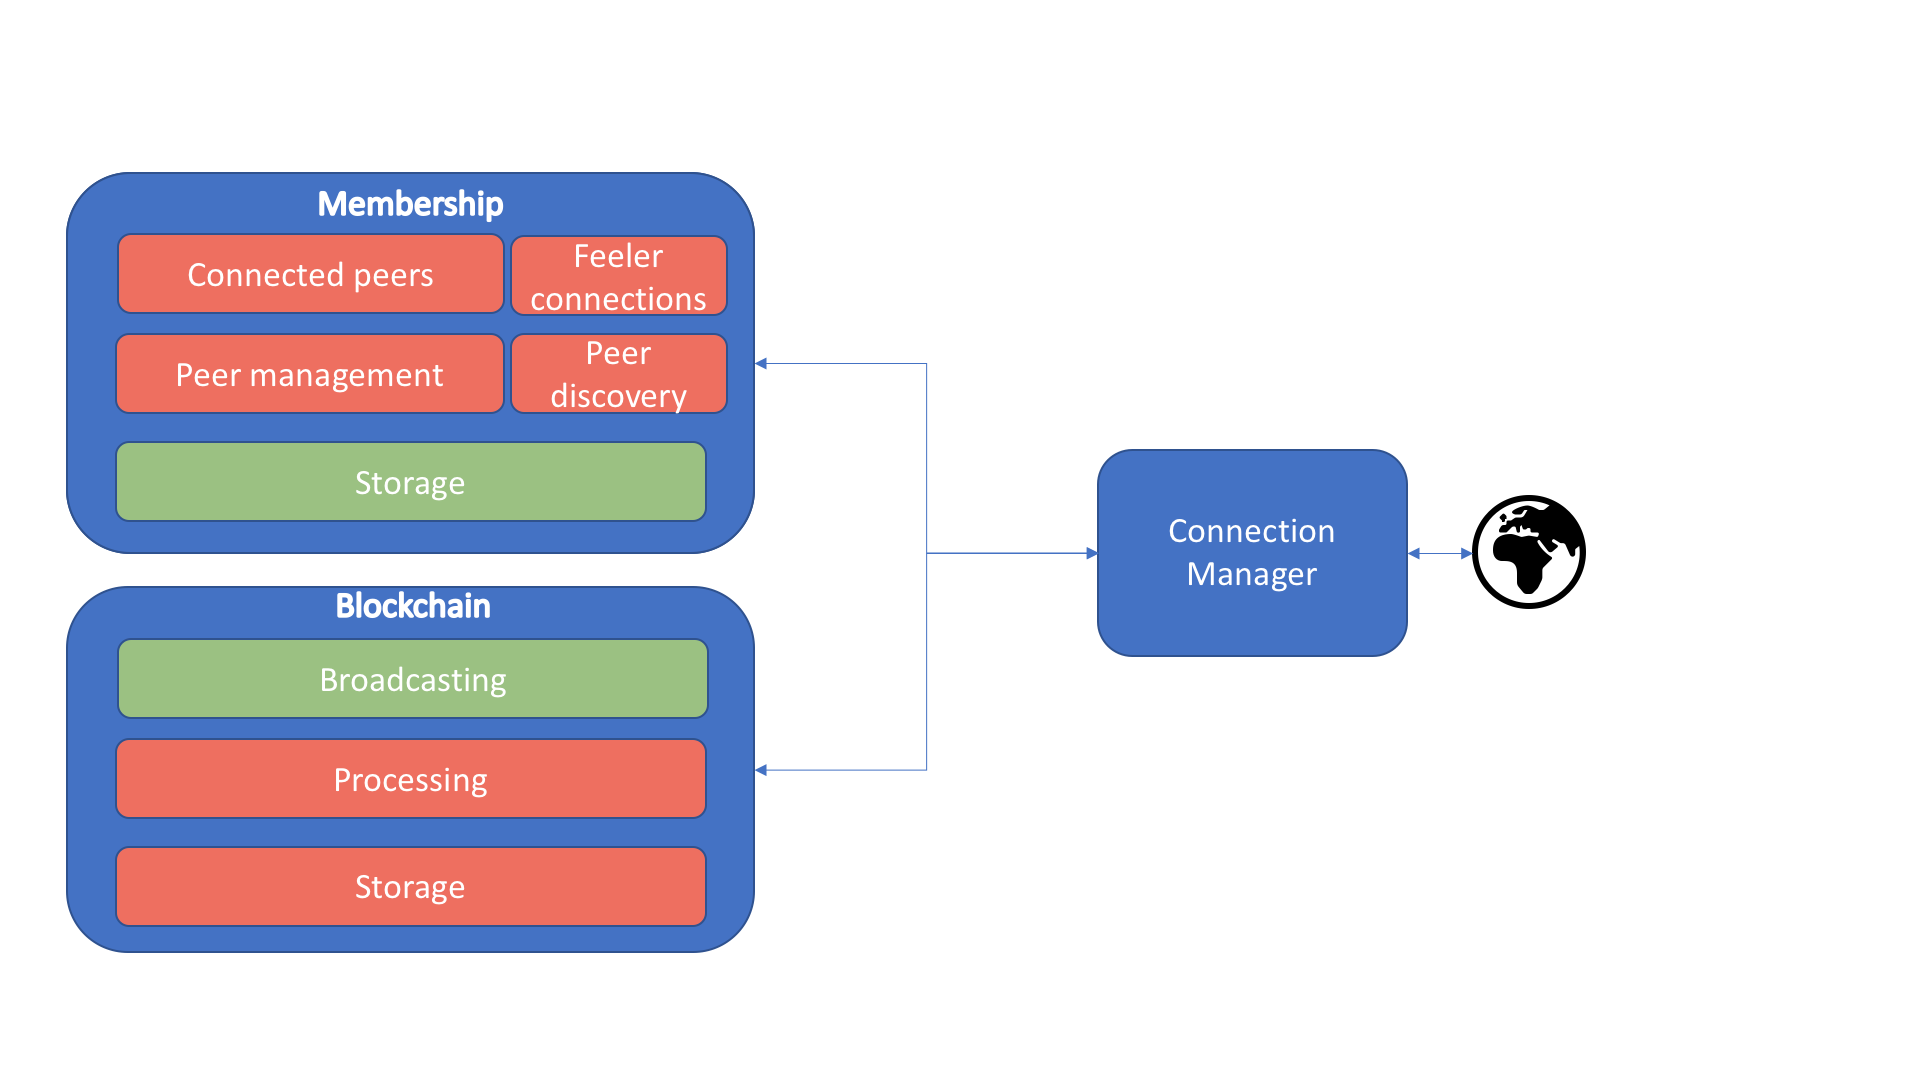
\includegraphics[scale=0.30]{figs/Architecture}
\caption{BitShield architecture}
\label{fig:bitshieldoverview}
\end{figure}

\textit{BitShield} is positioned between the \textit{Connection Manager} and the \textit{Peer Discovery} because those are the modules we have identified as the cause of the problems Bitcoin has.

In the rest of this section, we will cover each vulnerability individually and propose possible approaches that will help Bitcoin overcome these vulnerabilities.
In Section \ref{sec:evulne}, we will propose possible approaches to vulnerabilities that attackers can use to exploit Bitcoin. Whereas in Section \ref{sec:ivulne}, we will propose possible strategies to cope with behaviours that nodes inside the network might have to exploit Bitcoin and increase profit.
\subsection{External vulnerabilities}
\label{sec:evulne}

\paragraph*{\textbf{Information Eclipsing}}
Our approach to this problem is to implement the optimization in the propagation discussed in Section \ref{sec:ieclipsing}. To achieve this, when a node receives a block the verification of a block is split into two phases an initial difficulty check and a transaction validation. After the node validating that the block is valid through the first validation phase, the node would asynchronously broadcast \textit{inv} messages to his neighbours while performing the transaction validation. This will decrease the mean time it takes for a block to reach a node hence reducing the probability of forks happening. The drawback of this solution is that it only lowers the probability this problem happening.

%Our approach to this problem is to make the whole network aware of the existence of a fork. To achieve this, when a node received a block with the same height as the blockchain head, if that block was received soon after the node had received the current blockchain head then instead of not broadcasting it, the node would broadcast it allowing the full network to be aware of the fork. We believe this would lead to the end of the fork much faster. Because by making the full network aware of the fork nodes could choose which branch they would mine on.

It would also be interesting implementing the solution Ethereum used to solve this problem, \textit{Uncle Blocks} mentioned in Section \ref{sec:ieclipsing}. Where nodes include uncle blocks in future blocks strengthening the chain. They also reward nodes that found uncle blocks and nodes that add uncle blocks to their blocks which would compensate nodes that had their computational power wasted in a block that was not accepted. The problem with this approach is that it would have an increase in the block size and it would require more computational power from the nodes.

\paragraph*{\textbf{Partition attack}}
This attack is hard to protect against because the problem is not only related with Bitcoin but also with the protocol used by the ASes.

Hence, our aim is to use MACHETE and also make nodes establish some extra connections. In this approach, a node would have to establish extra connections while having into account the route that the packets were going to have then, nodes would also send certain key messages (like the \textit{inv} for instance) through multiple paths using the multipath approach of MACHETE. Nodes will use a tool like \textit{traceroute}\footnote{Diagnostic tool for displaying the route and measuring transit delays of packets across an Internet Protocol (IP) network.} to identify the best routes to avoid packets from passing always through the same AS. With this approach, a node is connected to the Bitcoin network through multiple AS and is able to communicate with different points of the network preventing the attack. A drawback of this approach would be the extra overweight imposed on the nodes to create the extra connections and send the extra messages.

\paragraph*{\textbf{Delay attack}}
This attack can be done in two different directions. Our approach is to address the problem in both directions as follows. Since this attack is targeted at a single connection that a node has with a neighbour of his. We will use a strategy like MACHETE and send multiple multiple block requests to different neighbours. With this strategy the attacker has to intercept more connections, this strategy also prevents the attack in both directions.

This solution might add overweight to the network because more request messages will be traversing the network. But if we compare the computational power wasted by the victim when being attacked with our solution, we believe that our solution will be better. Because not only are the messages small in size but also the victim will not be wasting computational power that could be used for strengthening the blockchain.

We also want to modify the behaviour of nodes in the \textit{N$\,\to\,$V} direction. Where once a node receives a corrupted block instead of staying idle it requests the block again. If the node fails 3 times to receive the block form that neighbour it drops the connection and asks for the block to another neighbour.

\paragraph*{\textbf{Mosquito attack}}
Our procedure to cope with this attack is to implement a system where every node analyzes the \textit{addr} messages that their neighbours share with them to identify if the neighbours are trying to attack them. The idea is if all neighbours are sharing the same set of addresses with a node through a period of time then the probability of them being malicious is high. If a node identifies a set of neighbours as malicious, he would ban those nodes and re-start its connection to the network. The disadvantages of this strategy are the extra computational power and memory wasted on the analysis of the \textit{addr} messages.

If we were to implement an approach where it costs a bit of the currency to send messages like Ripple or Ethereum. We would cope with this attack but it would require relevant changes to the Bitcoin protocol something that is not desirable by users in Bitcoin.

Implement authenticated messages for sharing IP addresses would also protect against the attack but it would require much more computational power and a system to distribute asymmetric key pairs.

\paragraph*{\textbf{51\% attack}}
For this attack, we are not going implement any solution in particular since this attack is always possible unless we control who joins the peer-to-peer network.

Still performing this attack in Bitcoin is very hard. Given the current competition in the mining community and the current size of the network, it would be very costly to gather 51\% of computational power.

\subsection{Internal vulnerabilities}
\label{sec:ivulne}
We will now address some of the solutions to the problems Bitcoin has with the behaviour of peers in the network and the way they connect between themselves.

\paragraph*{\textbf{Supernodes}}
To prevent this behaviour we are going to take advantage of the analysis that nodes are going to perform on \textit{addr} messages to prevent the mosquito attack. During the analysis, we will collect the number of times a node appears in those \textit{addr} messages and if a node reaches a certain number of appearances it is safe to presume that is a supernode. In this case, the node that identified the supernode will drop the connection with him and connect to another node. The disadvantages of this approach are once again the extra computational power required and also the possible increase of the mean time it takes for a block to propagate through all the network.

We could also introduce incentives towards a more random topology. An example of those incentives is the approach that Ripple and Ethereum used, where to send certain messages a node has to pay a fee. In our case to prevent supernodes, if a node exceeded a pre-established number of connections then for every extra connection the node would have to pay a fee in order to be able to sustain that connection. The problem with this approach is that we would have to modify the Bitcoin protocol something that is highly vetted against by the Bitcoin community.

\paragraph*{\textbf{Rational nodes}}
In Section \ref{sec:rpsummary}, we saw that in Bitcoin \textit{rational nodes} or \textit{selfish miners} do not behave like \textit{free riders} so we cannot implement directly approaches like the ones presented in before. In the context of file sharing, \textit{free riders} are nodes that would set their upload rate to low while having a high download rate. This is not applicable to Bitcoin because \textit{rational nodes} still work but they do not share the results of their work so that others waste their time and resources.

To prevent this we are going to implement a solution like LiFTinG \cite{guerraoui2010lifting} where nodes verify each other. In this solution, nodes analyze the messages their neighbours are broadcasting. The idea is for a node to analyze if a neighbour is broadcasting a new block right after receiving another block at the same height. If the neighbour did this a certain number of times then it would be safe to assume that that neighbour was a \textit{selfish node}. Nodes punish \textit{selfish nodes} by dropping the connection with them. The disadvantage of this solutions is the extra computational power required to perform these verifications and also the possibility of false positives.

Another possible approach that would minimize the impact of this behaviour is the implementations of uncle blocks. Because in this system node still gets rewarded for finding a block at the same height as the new blockchain head, up to a certain height difference.

\subsection{Summary}
Table \ref{fig:tabel2} summarizes the approaches we discussed above. As is possible to observe, there is no solution that fixes all the problems.

From Table \ref{fig:tabel2} there are some approaches that are not feasible to implement given the Bitcoin requirements for performance, those approaches are the \textit{encrypted messages} and \textit{authenticated messages}. Both approaches would require nodes to perform considerable more computations which would lower the profit of miners. Hence, these solutions would never be accepted by the Bitcoin community.

Other approaches like \textit{uncle blocks} and the \textit{implementation of fees} would be equally hard to implement given the relevant impact they would have on the protocol. Since \textit{uncle blocks} requires multiple nodes to be rewarded by the discovery of a new block and the \textit{implementation of fees} would require fees to be imposed on messages. Hence, both solutions would lower the profit of not only miners but also users and would be highly vetted against by the Bitcoin community.

However, there are still some approaches in Table \ref{fig:tabel2} that combined are able to cope with the multiple vulnerabilities while having a low impact on performance. Those approaches are the \textit{optimization in block propagation}, establishment of \textit{extra connections between nodes}, the use of \textit{MACHETE} to send messages through multiple paths, \textit{analysis of addr messagues} and the use of a \textit{LiFTinG approach} to cope with rational nodes. Although all these solutions combined will probably require more computational power from the nodes if we compare them with the approaches described before their impact is much lower.

% Please add the following required packages to your document preamble:
% \usepackage{graphicx}
\begin{table}[]
\centering
\resizebox{\textwidth}{!}{%
\begin{tabular}{l|c|c|c|c|c|c|c|c|c|c|}
\cline{2-11}
 & \begin{tabular}[c]{@{}l@{}}Uncle\\ Blocks\end{tabular} & \begin{tabular}[c]{@{}l@{}}Optimization\\ in block\\ validation\end{tabular} & \begin{tabular}[c]{@{}l@{}}Extra\\ connections\\ between\\ nodes\end{tabular} & MACHETE & \begin{tabular}[c]{@{}l@{}}Encrypted\\ messages\end{tabular} & \begin{tabular}[c]{@{}l@{}}Monitor\\ RTTs\end{tabular} & \begin{tabular}[c]{@{}l@{}}Analyze\\ addr\\ messages\end{tabular} & Fees & \begin{tabular}[c]{@{}l@{}}Authenticated\\ messages\end{tabular} & \begin{tabular}[c]{@{}l@{}}LiFTinG\\ approach\end{tabular} \\ \hline
\multicolumn{1}{|l|}{\begin{tabular}[c]{@{}l@{}}Information\\ Eclipsing\end{tabular}} & $\bigcirc$ & $\bigcirc$ &  &  &  &  &  &  &  &  \\ \hline
\multicolumn{1}{|l|}{\begin{tabular}[c]{@{}l@{}}Partition\\ Attack\end{tabular}} &  &  & $\bigcirc$ & $\checkmark$ & $\checkmark$ & $\bigcirc$ &  &  &  &  \\ \hline
\multicolumn{1}{|l|}{\begin{tabular}[c]{@{}l@{}}Delay\\ Attack\end{tabular}} &  &  & $\bigcirc$ & $\checkmark$ & $\checkmark$ & $\checkmark$ &  &  & $\bigcirc$ &  \\ \hline
\multicolumn{1}{|l|}{\begin{tabular}[c]{@{}l@{}}Mosquito\\ Attack\end{tabular}} &  &  &  &  &  &  & $\checkmark$ & $\checkmark$ & $\checkmark$ &  \\ \hline
\multicolumn{1}{|l|}{51\% Attack} & $\bigcirc$ & $\bigcirc$ & $\bigcirc$ &  &  &  &  & $\bigcirc$ &  &  \\ \hline
\multicolumn{1}{|l|}{Supernodes} &  &  &  &  &  &  & $\checkmark$ & $\checkmark$ &  &  \\ \hline
\multicolumn{1}{|l|}{\begin{tabular}[c]{@{}l@{}}Rational\\ nodes\end{tabular}} & $\bigcirc$ &  & $\bigcirc$ &  &  &  &  & $\bigcirc$ &  & $\checkmark$ \\ \hline
\end{tabular}%
}
\caption{Solutions to the problems. \\ $\checkmark$ - Protects against the problem \\ $\bigcirc$ - Helps protect against the problem}
\label{fig:tabel2}
\end{table}

\section{Melhorando a Propagação das Transacções}

Nesta secção propomos um conjunto de alterações ao mecanismo de propagação de transacções na Bitcoin com o objectivo o tornar mais eficiente, nomeadamente, de reduzir o número de anúncios redundantes que cada nó da rede recebe. A nossa proposta é fundamentada nas seguintes observações:

\begin{itemize}
\item Actualmente, os nós recebem em média $3.33$ anúncios para cada transacção (quando bastaria receberem no máximo um único para garantir a recepção da transacção).
\item A rede possui dois mecanismos complementares para propagar transacções: a troca de anúncios (usada antes da transacção estar inserida num bloco) e a troca de blocos (que implicitamente anunciam as transacções que lhe estão associadas).
\item Por razões históricas, o segundo mecanismo é mais eficiente, pois todas as transações em falta num nó são enviadas numa única mensagem (enquanto que o mecanismo de propagação epidémica inicial, obriga a troca de uma mensagem individual para cada transacção).
\item A rede Bitcoin não tem requisitos estritos de latência para a propagação das transações, uma vez que a taxa de geração de blocos é significativamente mais lenta que o processo de propagação epidémico (em média, é gerado um novo bloco a cada 10 minutos).
\item Os mineiros são uma fracção reduzida do número total de nós. Apesar de ser fundamental que as transacções sejam conhecidas pelo mineiros, o protocolo de disseminação não distingue os mineiros dos restantes nós.
\item No protocolo epidémico actualmente usado na Bitcoin, os anúncios são escalonados para serem propagados para todos os vizinhos que o nó conhece (cerca de 125).
Este valor é substancialmente maior do que o valor teórico dos protocolos de disseminação epidêmicos que sugere que, mesmo na presença de faltas, basta propagar informação para um número de vizinhos que é aproximadamente logarítmico com o tamanho da rede~\cite{epidemicDiss}. Para o tamanho atual da rede, que possuí cerca de $10~000$ nós bastaria portanto propagar para $ ln(10~000) \approx 10$ vizinhos.
\end{itemize}

O principal desafio é reduzir a quantidade de anúncios redundantes trocada na rede e, ao mesmo tempo, assegurar que as transações chegam aos nós mineiros.
A intuição da abordagem proposta é enviesar o processo de propagação na direcção dos mineiros mais produtivos na rede sem, no entanto, deixar de assegurar que a informação é também propagada por caminhos alternativos para os restantes nós e mineiros.
Isto é concretizado através de duas modificações ao protocolo.
A primeira consiste em adicionar um novo campo às mensagens que propagam os blocos que indica o número de saltos que o bloco dá na rede.
Isto permite que cada nó fique a saber a que distância está o mineiro que gerou esse bloco.
Esta informação é codificada num inteiro e portanto tem um impacto negligenciável no tamanho total do bloco que ronda 1 MB\@.
A segunda modificação consiste em identificar localmente, com o passar do tempo, qual o caminho para os mineiros mais próximos e enviar a propagação de anúncios preferencialmente por estes caminhos.
Note-se que a partir do momento em que uma transacção é incluída num bloco, o processo de propagação por troca epidémica de anúncios deixa de ser relevante.

%\subsection{Seriação dos Vizinhos}

%Como foi referido acima, a estratégia proposta para poupar largura de banda pressupõe que cada nó descobre quais os melhores caminhos para chegar aos mineiros mais próximos. Isto é conseguido seriando o vizinhos por um critério de proximidade aos mineiros. Os vizinhos mais perto dos mineiros ficam listados no topo da tabela e os mais afastados são seriados no fundo da tabela.

%Para obter esta classificação, cada nó mantém, para cada vizinho, três variáveis: \textit{n}, o número total de blocos que recebeu desse vizinho; \textit{k} a distância acumulada desses blocos até aos mineiros que o produziram; e finalmente \textit{a}, o número total de blocos recebidos.
%Para permitir actualizar \textit{k}, associamos ao processo de propagação de um novo bloco, um contador que regista quantos saltos o bloco deu na rede Bitcoin (este campo é incrementado sempre que um nó reencaminha o bloco). Com base nestas variáveis, a classificação dos vizinhos num determinado intervalo de tempo \textit{T} é feita de acordo com a seguinte fórmula (em que os valores de $k$, $a$ e $n$ são os acumulados no período $T$):

%\[ \mbox{class}^{T}= (\dfrac{k^{T}}{n^{T}} + a^{T}-n^{T}) \]

%Esta caracterização evita que nós com baixa capacidade de mineração que geram blocos muito esporadicamente, fiquem indefinidamente com uma boa classificação.
%Isto é relevante pois uma percentagem dos blocos é gerada por nós com baixa capacidade de mineração, que queremos evitar  aleatórios assim, se enviássemos as nossas transações sempre para esses nós elas poderiam demorar muito tempo até aparecerem em blocos podendo até ficarem perdidas.
%Desta forma, balanceamos não só os vizinhos que têm melhor rácio distancia aos mineiros/número de blocos providenciados, mas também conseguimos ter em conta o número total de blocos que esse vizinho nos forneceu relativamente ao número total de blocos recebidos.

%Uma vez que a classificação de cada um dos vizinhos se vai alterando ao longo do tempo, o valor usado para seriar os vizinhos é uma média deslizante da classificação instantânea acima referida, dada por:

%\[ \mbox{class}^t = (1-\alpha) \cdot \mbox{class}^{t-1}  + \alpha \cdot \mbox{class}^{T} \]

%O factor $\alpha$ existe para evitar que vizinhos de  mineiros que já tenham sido extremamente activos no passado mas que no tempo actual já não o são, permanecem para sempre no topo da tabela. Nas nossas experiências usamos $\alpha=0.3$ e \textit{T} é configurado como sendo um intervalo de 4 horas.

%Cada vez que um nó recebe um bloco de um vizinho, a classificação é atualizada conforme descrito no Algoritmo~\ref{alg:class}.
%<++> os seguintes passos vão acontecer de forma a mantermos uma lista com os $m$ vizinhos com menor valor de classificação:



%Na nossa solução, de forma a que um nó consiga determinar para qual dos seus vizinhos deve enviar transações vai somar o inteiro que indica o número de saltos que o bloco dá na rede a uma variável associada ao vizinho de quem recebeu o bloco. Esta variável vai ser depois dividida pelo número total de blocos recebidos através desse vizinho de modo a possamos associar um valor de proximidade ao mineiro a cada vizinho. Visto que o campo presente nas mensagem que propagam os blocos deve ser incrementado sempre que um nó envia o bloco para um dos seus vizinhos é evidente que os vizinhos com o menor valor de proximidade a mineiros vão ser os vizinhos que teoricamente estarão mais perto dos mineiros.

%\subsection{Propagação Enviesada}
%\label{sec:propagacao}
%Dado que o nosso objectivo é fazer com que as transações que conhecemos cheguem rapidamente aos mineiros podemos utilizar o mecanismo descrito na secção anterior para atingir este objectivo. Assim se estivéssemos perante uma rede onde todos os nós cumpriam com o protocolo e os caminhos fossem resilientes o suficiente poderíamos apenas enviar as transações que recebíamos para o nosso vizinho que tivesse menor valor de classificação e inevitavelmente essas transações seriam adicionadas a um bloco.

%No entanto, para além das falhas por paragem, temos de ter em conta que os nós podem manipular o $k$ enviado aos seus vizinhos, colocando-o a zero.
%Deste modo seriam erradamente priorizados e poderiam ficar em vantagem de duas maneiras: conhecer as transações mais cedo, e não propagar as transações recebidas.
%ara evitar este problema, além de disseminarmos as transações para os vizinhos com mais prioridade, enviamos também para um conjunto aleatório de vizinhos, conforme descrito no Algoritmo~\ref{alg:diss}. Desta forma asseguramos que as transações continuam a ser disseminadas pelo resto da rede mesmo que tenhamos como vizinho um nó malicioso.
%Desta forma sempre que um nó receber uma transação vai enviar esta para o conjunto de vizinhos com melhor classificação\textit{m} e vai concorrentemente enviar a transação para um conjunto de nós escolhidos ao acaso \textit{a} tal como descrito no algoritmo abaixo:



%O valor de \textit{pi} (Push inicial) indica se quando uma transação é gerada deve ser enviada apenas para \textit{m} e \textit{a} ou para todos os vizinhos.
%e \textit{a} enviar para todos os seus vizinhos.
%Desta forma os valores de \textit{tamanho\_m}, \textit{tamanho\_a} e \textit{pi} podem depois ser alterados para obtermos diferentes padrões de propagação.
%Na Secção~\ref{sec:calibracao} discutimos as diferentes configurações testadas.

%\subsection{Concretização}

%O nosso objectivo de longo prazo é vir a incluir uma versão da nosso algoritmo na distribuição do Bitcoin. No entanto, esse processo é moroso e requer evidências das vantagens da solução. Não sendo exequível fazer experiências com milhares de nós num ambiente real com uma versão alterada do cliente Bitcoin, tivemos de recorrer a simulação para avaliar o nosso algoritmo.

%Para criarmos uma simulador fiel ao cliente original, começámos por fazer alterações ao cliente da \textit{Bitcoin Core} (cliente mais usado) para recolhemos estatísticas em relação às mensagens trocadas pelos clientes que usam a distribuição por omissão. Desta forma alteramos o cliente para que este capturasse as seguintes informações:
%\begin{itemize}
%\item anúncios de transações;
%\item transações que recebidas;
%\item transações presentes em blocos compactos que o nó não possuía e tinha de pedir de forma a poder reconstruir o bloco.
%\end{itemize}
%Uma vez feitas as alterações lançamos o cliente numa zona da rede não protegida onde ficou ligado à rede Bitcoin durante um mês. Com as métricas que recolhemos ficamos com informação de referencia para poder calibrar o simulador.

%As simulações recorrem a simulador de eventos discreto, programado em Python,  que funciona por ciclos. Em cada ciclo os nós verificam se têm eventos para processar e, em caso afirmativo, executam o código que processa esse evento. Este código mimetiza o comportamento de um cliente Bitcoin (foram concretizadas duas versões, uma que tem o comportamento padrão e outra que corre as nossas modificações). Como resultado de processar um evento, um nó pode gerar novos eventos (que serão processados em ciclos futuros). Cada ciclo do simulador corresponde a um segundo de tempo real.

%Uma simulação começa com a criação de uma rede de nós que pode ser carregada de um ficheiro ou criada de raiz. Na rede criada, cada nó tem  8 vizinhos \textit{de escoamento} que são escolhidos aleatoriamente entre todos os nós. Mais nós podem ser adicionados a esta lista de vizinhança caso estabeleçam uma ligação com o nó ficando estes nós marcados como \textit{incidentes}, nunca podendo um nó estabelecer mais do que 125 conexões.
%São também escolhidos ao acaso um conjunto de mineiros que mantêm o rácio mineiros número de nós na rede.  De seguida o simulador cria uma lista com os nós que vão gerar transações em cada ciclo. Depois da rede estar criada a simulação começa, onde cada nó sequencialmente executa a função \textit{CICLO}, verificando se necessita de gerar transações, de gerar um bloco ou de enviar anúncios de transações aos seus vizinhos.

%\begin{itemize}
%\item No momento de criar uma transação, o nó de origem regista este evento um contador global que captura quantas transações já foram criadas no sistema, adiciona a transação à sua lista de transações conhecidas e coloca essa transação nas filas de anúncios a enviar aos seus vizinhos. Cada transação tem o tamanho de  700 bytes.
%\item No momento de criar um bloco, um nó determina qual será o ciclo em que o cripto puzzle será resolvido. Após correr esta função vai buscar à sua lista de transações \textit{pendentes} transações até encher o bloco (1428 transações) ou ficar sem transações  \textit{pendentes}. Finalmente vai criar o bloco, adicioná-lo à sua lista de blocos e anunciá-lo aos seus vizinhos.
%\item Cada nó mantém, para cada um dos seus vizinhos, uma lista de anúncios \textit{prontos} a enviar. Para enviar anúncios aos seus vizinhos, o nó começa por calcular, para cada vizinho, qual vai ser o próximo ciclo em que deve realizar a transmissão (a propagação dos anúncios é atrasada deliberadamente, para reduzir o tráfego de controlo). Quando esse instante chegar, retira um anúncio da lista de \textit{prontos}, verifica se o vizinho ainda não conhece esse anuncio e, caso ele não o conheça adiciona esse anuncio, a uma lista de anúncios a transmitir. Este processo é repetido até a lista de anúncios \textit{prontos} ficar vazia ou a lista de anúncios a enviar chegar ao tamanho limite de  35. No fim deste processo,  a lista de anúncios é enviada.
%\end{itemize}

%No simulador,  concretizámos o funcionamento das principais mensagens trocadas por nós após terem estabelecido ligações, essas mensagens são mensagens \textsl{Inv, GetHeaders, Headers, GetData, Block, CmpctBlock, GetBlockTX, BlockTX} e \textsl{TX} . Vamos agora explicar o  comportamento de um nó quando recebe cada uma destas mensagens.

%Quando um nó recebe uma mensagem de anúncios \textsl{INV}, vai percorrer todos os anúncios nessa mensagem e, para cada anúncio, realiza os seguintes passos:
%\begin{itemize}
%\item Verifica qual o tipo de anúncio (existem dois tipos de anúncios, os que anunciam blocos e os que anunciam transações);
%\item Atualiza o inventário do vizinho que enviou a mensagem, registando a informação anunciada;
%\item Verifica se já possui a informação anunciada. Caso não a possua, vai adicionar essa informação a uma lista de informação a pedir.
%\end{itemize}

%No depois de ter iterado por todos os anúncios, o nó envia uma mensagem de \textsl{GetHeaders} caso o anúncio tenha sido de blocos e envia uma mensagem \textit{GetData} caso o anúncio tenha sido de transações.

%Quando um nó recebe uma mensagem de pedido de informação \textsl{GetData, GetHeaders}, vai atualizar o inventário do vizinho que lhe enviou a mensagem e vai responder com a informação requisitada.

%Quando um nó recebe uma mensagem de \textsl{Headers}, o nó itera sobre todos os cabeçalhos incluídos e adiciona-os à sua cadeia de cabeçalhos. Caso não conheça o antecessor de um bloco, o nó requisita também o cabeçalho respectivo. Depois de adicionar os cabeçalhos à cadeia de cabeçalhos, requisita os blocos associados a esses cabeçalhos com uma mensagem \textsl{GetData}.

%Quando um nó recebe uma mensagem de \textsl{TX}, vai atualizar o inventário do vizinho e seguidamente caso não possua a transação, adiciona-a à sua lista de transacções \textit{pendentes} e invoca uma função, designada por \textit{push\_to\_send}, para disseminar essa transação aos vizinhos que ainda não a possuem.

%Quando um nó recebe um bloco compacto através de uma mensagem \textsl{CmpctBlock}, o nó verifica se já possui esse bloco e caso já o possua  atualiza apenas o inventário do vizinho que lhe enviou o bloco. Caso não possua o bloco, verifica se têm todas as transações presentes no bloco;  se não possuir uma ou mais transações requisita-as com uma mensagem de \textsl{GetBlockTX} e coloca o bloco numa lista de blocos parcialmente construidos. Assim que receber a resposta à mensagem de requisito de transações acaba de reconstruir o bloco e inicia o processamento do novo bloco. Quando um nó recebe um bloco completo através de uma mensagem \textsl{Block}, caso não o possua vai processá-lo.

%O processamento de um bloco começa por atualizar o inventário de blocos. Caso o novo bloco seja posterior ao bloco mais recente que o nó conhece, atualiza-se o estado do livro razão dá-se inicio ao cálculo de um novo bloco. Por fim,  antes de se iniciar a disseminação do bloco,  removem-se as transações incluídas no bloco da lista de transações \textit{pendentes}. Durante a disseminação de um bloco, se o vizinho possuir o bloco anterior ao novo bloco então envia-se o novo bloco através de uma mensagem \textsl{CmpctBlock}; caso contrário envia-se uma mensagem de \textsl{Header}.

%A versão modificada, que suporta o nosso algoritmo, executa a seguinte funcionalidade adicional. Em primeiro lugar, é associado ao processo de propagação de um novo bloco, um contador que regista quantos saltos o bloco deu na rede Bitcoin até chegar ao nó que o está a receber. Isto permite que cada nó mantenha uma estimativa da sua distância, em número de saltos, para cada mineiro e quais os vizinhos que fazem parte do caminho para esses mineiros. Como os blocos não percorrem sempre o mesmo percurso, esta distância poderá variar cada vez que um bloco é produzido, pelo que cada nó vai mantendo uma média deslizante desta distância, que é actualizada sempre que chega um novo bloco. Cada nó mantém também informação de quantos blocos foram gerados por cada mineiro. Estas duas informações permitem estabelecer uma ordenação dos vizinhos, em que os vizinhos mais perto dos mineiros mais produtivos são seriados no topo da tabela, e os vizinhos afastados desses mineiros são relegados para o fim da tabela. Esta seriação é posteriormente usada para enviesar o processo de propagação de transacções: sempre que um nó executar a função \textit{push\_to\_send} para anunciar novas transações, vai apenas adicionar a transacção à lista anúncios \textit{pendentes} de alguns dos vizinhos, de acordo com o algoritmo descrito anteriormente.
